\documentclass[adobefonts, a4paper]{ctexart}

\usepackage[top=1.2in, bottom=1.2in, left=1in, right=1in]{geometry}
\usepackage{minted, graphicx, hyperref}

\hypersetup{colorlinks=true, linkcolor=blue}

\title{操作系统实验报告3}
\author{蔡日骏\quad12348003}

\begin{document}
\maketitle

\section{概述}
本次实验内容与我在实验2中完成的基本一样,本次只是将内核和部分用户程序用C语言重写。
因此这里不在赘述系统的基本架构。本次实验的报告主要介绍对实验2的改进。

\section{改进}
\subsection{文件系统}
在本次的实现中,用户程序文件的列表不再简单地保存在MBR中,而是放在某个扇区中,并把
扇区的线性逻辑地址记录在MBR中。可记录的文件数量从实验2的4个扩展到128个。

\subsection{函数库}
由于当前版本的gcc已不再支持16位实模式,编译时只能加入\verb|.code16gcc|伪指令让汇编
器加入16位指令前缀来实现实模式运行,但是函数调用约定仍然是32位的。因此,本次实验中
加入了32位C调用约定版本的函数库\verb|utils_32cc.o|。但是最新版的gcc传参数时默认按
16字节对齐,这里为了节省内存而选用了4字节对齐。编译时需要给gcc传入\verb|-mpreferred-stack-boundary=2|
参数。

此外,函数库的C头文件\verb|utils_32cc.h|中还提供了一些额外的函数以方便使用。

\subsection{用户程序公共头文件}
为了方便使用C语言开发用户程序,提供了一个\verb|user_program.h|文件,使用内联汇编
完成寄存器保护和跳转工作。

\subsection{其他}
本次实验中修复了上一版本中的一些漏洞。主要有:
\begin{itemize}
    \item 控制台中退格时会删掉提示符
    \item 某些库函数对寄存器的保护不符合C调用约定
    \item \verb|read_disk|函数无法访问起始地址位于第二磁头的位置
\end{itemize}

\section{编译说明}
直接运行

\begin{minted}{bash}
    $ make all
\end{minted}

即可。

\section{运行截图}

\begin{figure}[htp!]
    \center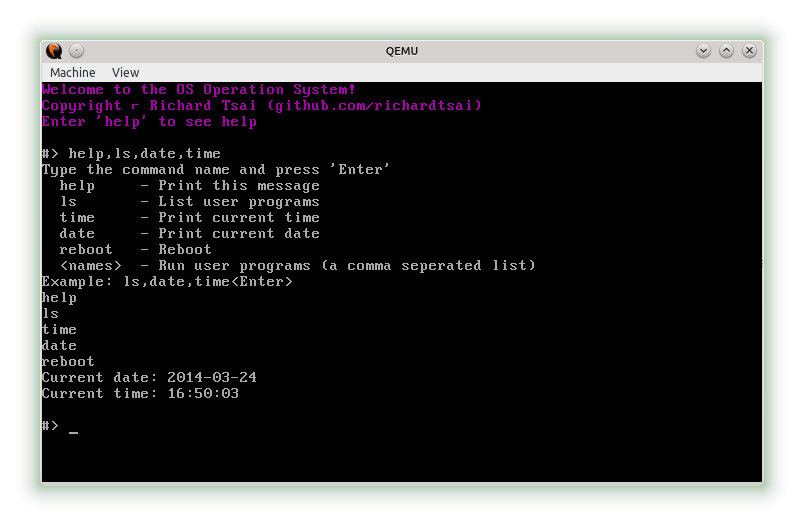
\includegraphics[scale=0.75]{demo}
\end{figure}

\end{document}
